\documentclass[12pt,letterpaper, spanish]{article}
\usepackage[spanish]{babel}
%\oddsidemargin=0cm
%\topmargin=-1cm
\usepackage[latin1]{inputenc}
\usepackage{graphicx}

\begin{document}

{\Huge {\rm { \bf Instituto Politecnico Nacional}}}\\
\begin{center}
{\huge {\rm {\em Escuela Superior de C\'omputo}}} \\
\end{center}
\begin{center}
{\Large {\em Tecnolog\'ias para la Web}}\\
\end{center}
\begin{center}
{\Large Alejandro Hern\'andez Hern\'andez}\\
\end{center}
\begin{center}
{\huge {\bf PR\'ACTICA 2}}
\end{center}

\newpage
{\Huge{\rm {\bf Introducci\'on}}}
%aqui algo como introduccion
\\\\En la practica, se comenz\'o el uso de los archivos {\bf xhtml}, asi como el uso de las hojas de estilos {\em css} para el dise\~no de la pagina web personal el cual tiene contenido variado, que va desde informacion un tanto personal, hasta pasatiempos y contenido sin sentido.\\
\\Ademas, de una peque\~na secci\'on que muestra un tutorial de {\bf {\em html}}, con una peque\~na descripcion de la pagina y la parte m\'as basica del lenguaje {\em html}

\newpage
{\Huge {\rm {\bf Desarrollo}}}

\begin{flushleft}
Se sobreentiende que el servidor debe de estar arriba.\\
Lo primero que debemos de definir es nuestro {\bf {\em 'layout'}} o {\bf {\em 'boceto'}} de la pagina web. En mi caso, el layout fue el siguiente:\\
\vspace{-5mm}
%aqui la imgn
\begin{center}
\begin{figure}[h]
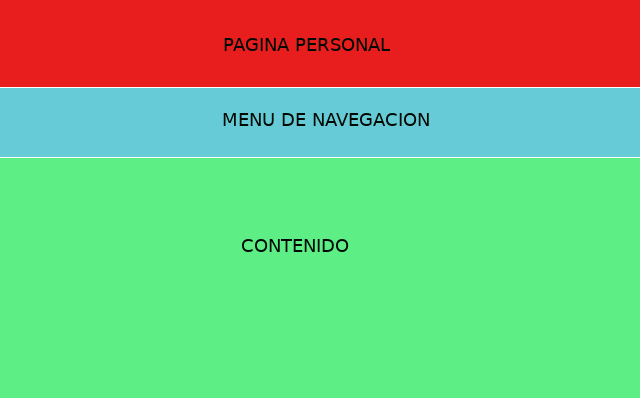
\includegraphics[width=400pt]{./imgs/plantilla.png}
\vspace{-8mm}
{\em{\caption {Layout}}}\label{figure 1}
\end{figure}
\end{center}
\vspace{-1cm}
Una vez definido el layout, se interpreta a codigo html, entonces el layout queda:
%la imgn
\newpage
\vspace{-3cm}
\begin{center}
\begin{figure}[h!]
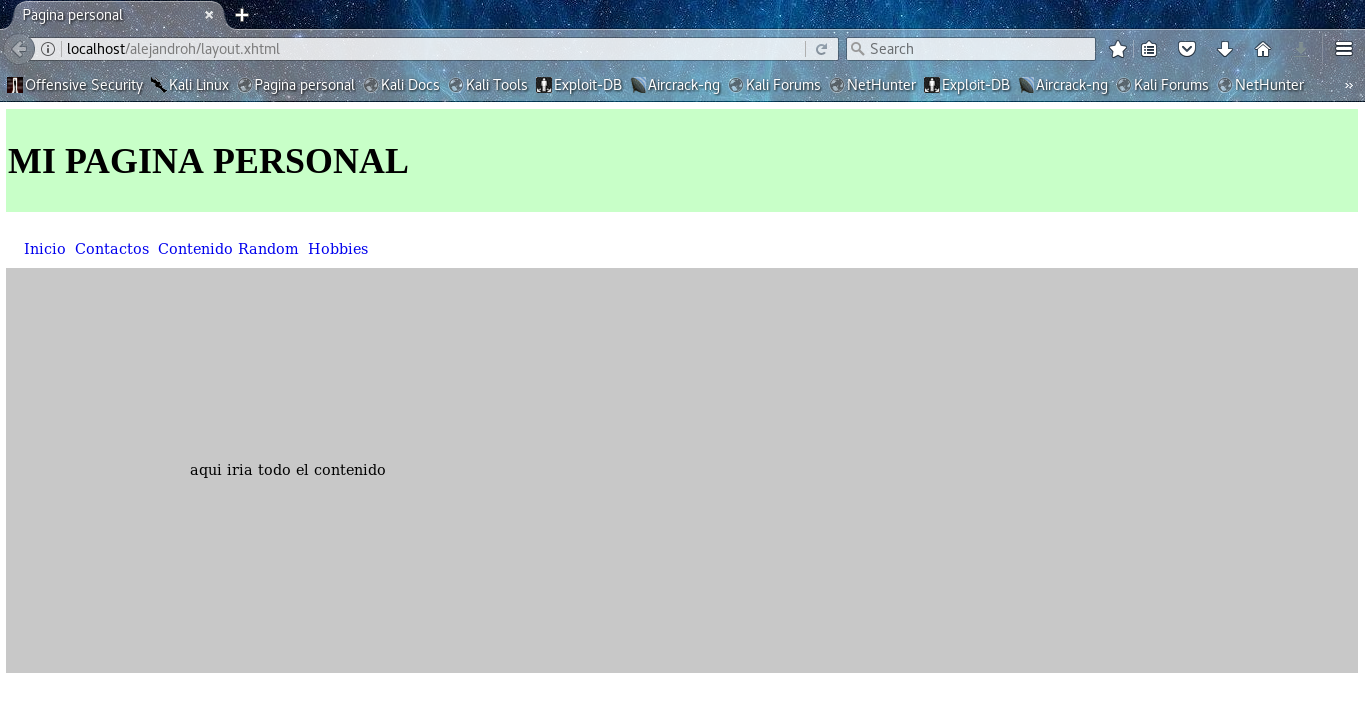
\includegraphics[scale=0.3]{./imgs/layout.png}
\vspace{-10mm}
{\em{\caption {Layout codificado}}}\label{figura 2}
\end{figure}
\end{center}
\vspace{-1cm}
Puesto que ya tenemos el layout codificado, y en el menu aparecen 5 items, repetir\'e 4 veces el layout. El ultimo item, {\em Tutorial html}, tendr\'a otra vista diferente.\\
Una vez hecho esto, nos dedicaremos a incluir el contenido en nuestros layouts, en mi caso, el 1er layout es el inicio, aqui se incluye el nombre y la ocupacion actual, incluyendo los logotipos correspondientes, y llamando al archivo {\em index.}{\bf{\em xhtml}}
%la imgn
\begin{center}
\begin{figure}[h!]
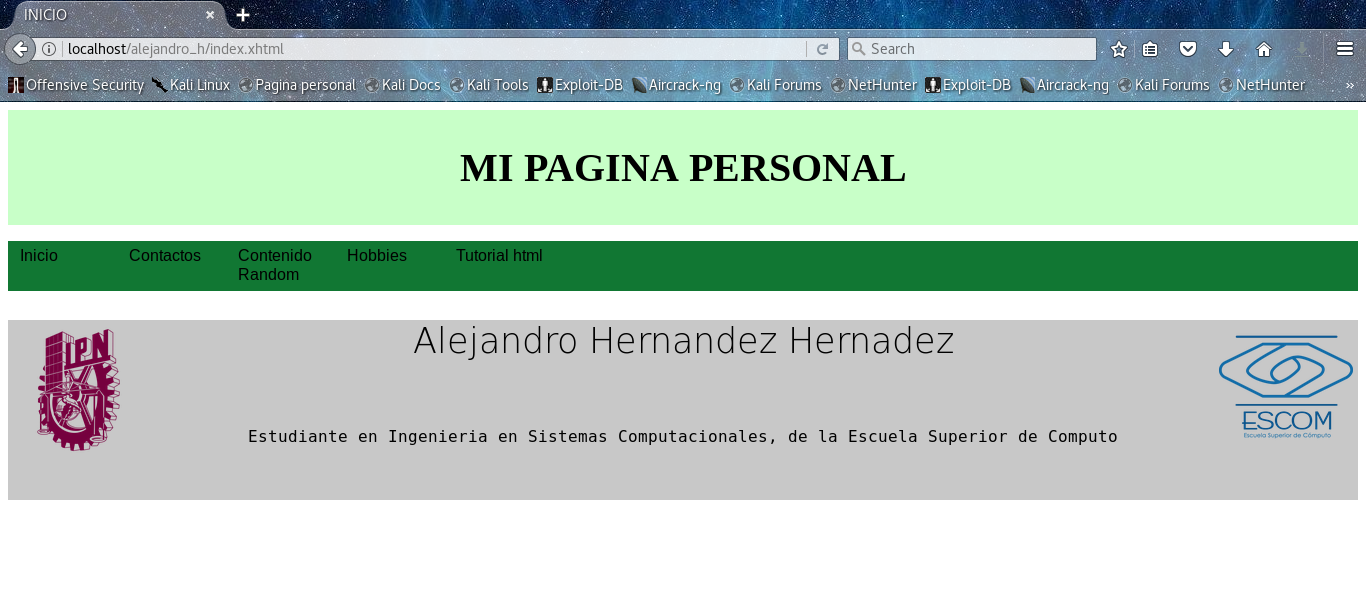
\includegraphics[scale=0.3]{./imgs/inicio.png}
\vspace{-2cm}
{\em{\caption {inicio}}}\label{figura 3}
\end{figure}
\end{center}
\vspace{-1cm}

Al segundo layout, le llamar\'e {\em contactos.}{\bf {\em xhtml}}:
\newpage
\begin{center}
\begin{figure}[h!]
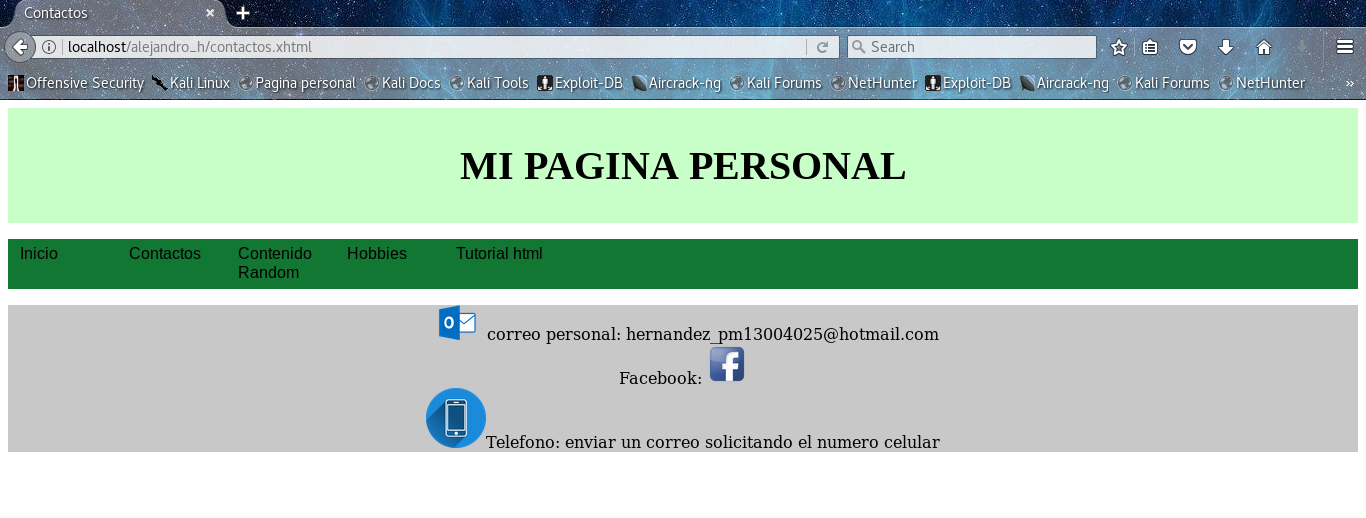
\includegraphics[scale=0.3]{./imgs/contactos.png}
\vspace{-15mm}
{\em{\caption {contactos}}}\label{figura 4}
\end{figure}
\end{center}
\vspace{-1cm}
Al 3er layout, le denominar\'e {\em random.}{\bf {\em xhtml}}
\begin{center}
\begin{figure}[h!]
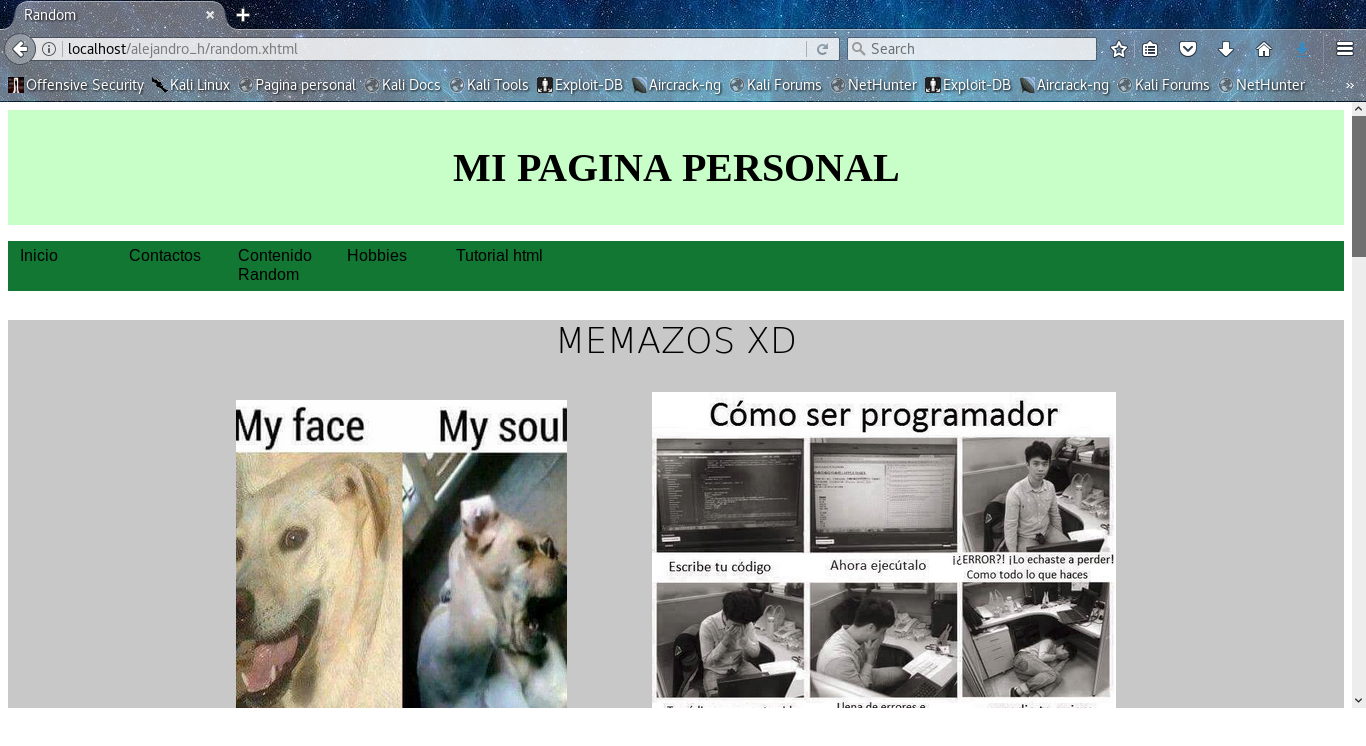
\includegraphics[scale=0.3]{./imgs/random.png}
\vspace{-10mm}
{\em{\caption {contactos}}}\label{figura 5}
\end{figure}
\end{center}
\vspace{-1cm}
Al 4to layout, le llamar\'e {\em hob.}{\bf {\em xhtml}}
\newpage
\vspace{-15mm}
\begin{center}
\begin{figure}[h!]
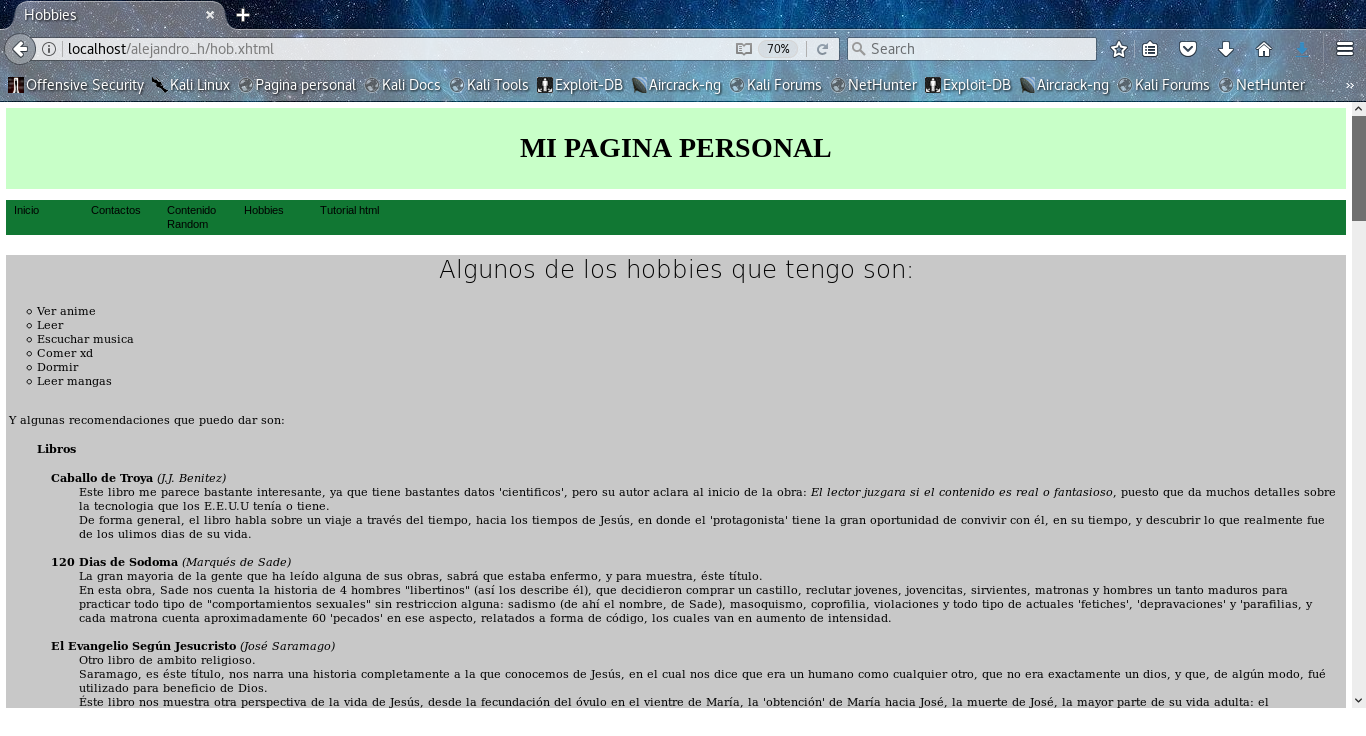
\includegraphics[scale=0.3]{./imgs/hob.png}
\vspace{-10mm}
{\em{\caption {hobbies}}}\label{figura 6}
\end{figure}
\end{center}
\vspace{-1cm}

Por \'ultimo, agregaremos el {\em Tutorial de html}, pero solo agregaremos unas cuantas etiquetas, dado que si se agregan todas, es demasiado contenido y me llevar\'ia demasiado tiempo.\\
Entonces, tendremos como dise\~no o layout:
\vspace{-5mm}
\begin{center}
\begin{figure}[h!]
\hspace{2cm}
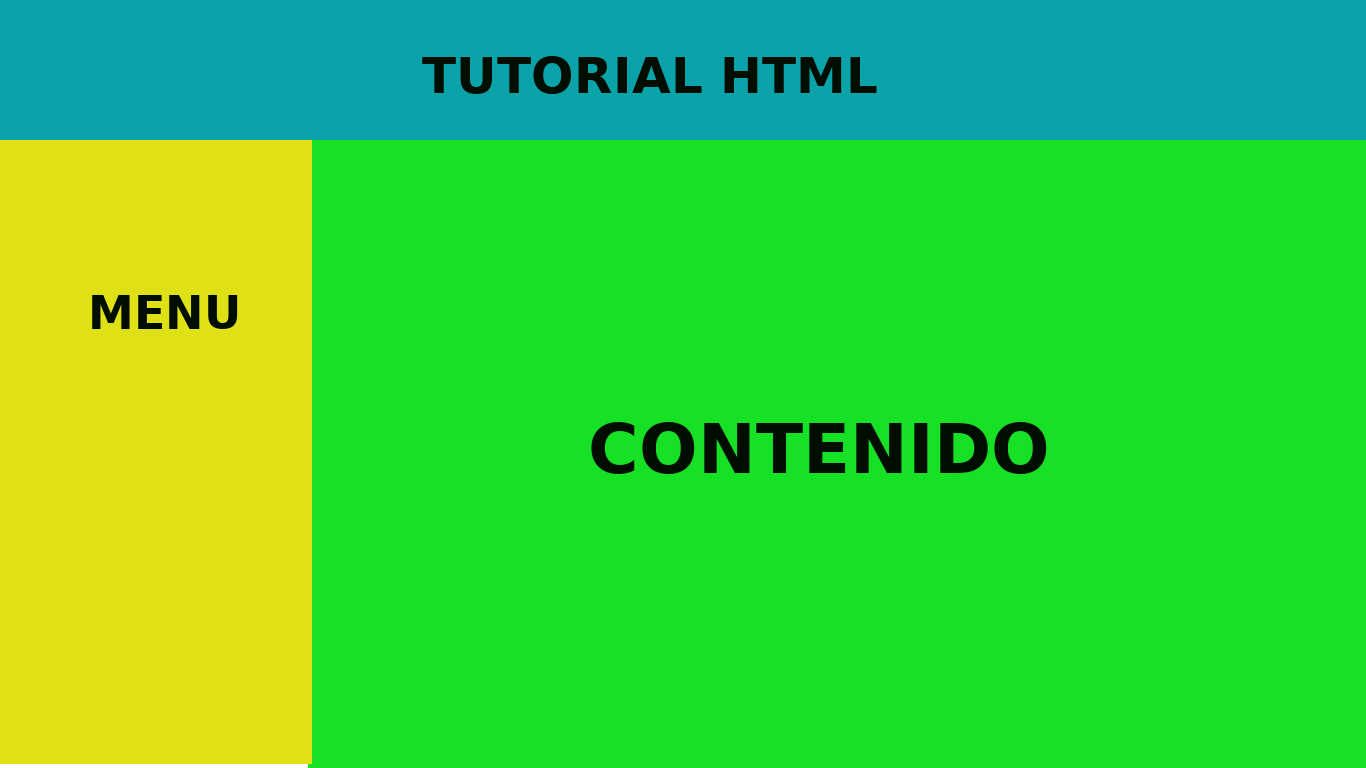
\includegraphics[scale=0.2]{./imgs/tutohtml.png}
\vspace{-5mm}
{\em{\caption {layout tutorial html}}}\label{figura 7}
\end{figure}
\end{center}
\vspace{-1cm}
\newpage
Y codificando el dise\~no anterior, se ver\'a:
\vspace{-5mm}
\begin{center}
\begin{figure}[h!]
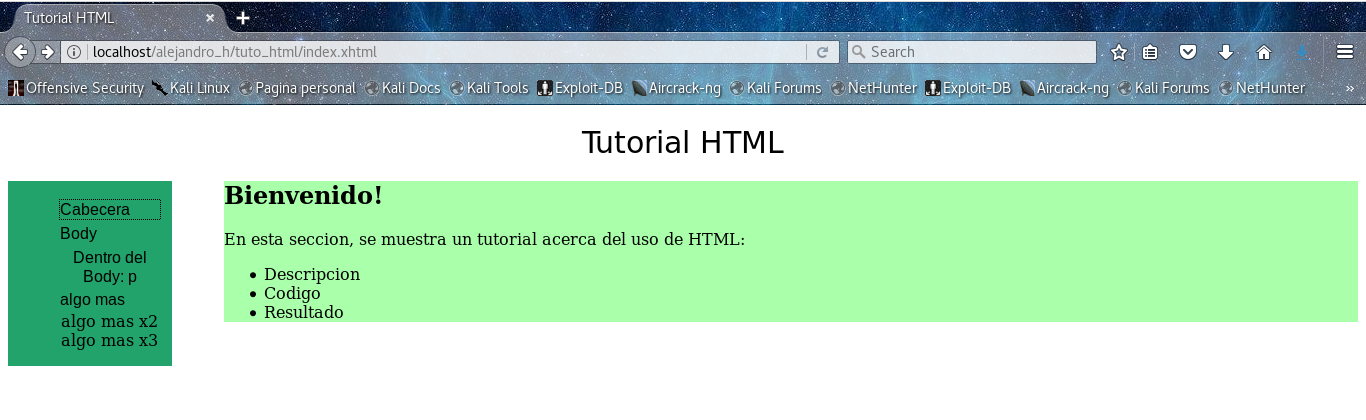
\includegraphics[scale=0.3]{./imgs/tuto.png}
\vspace{-10mm}
{\em{\caption {Inicio Tutorial html}}}\label{figura 8}
\end{figure}
\end{center}
\vspace{-1cm}
Las etiquetas que se utilizar\'an son las basicas:\\
\begin{verbatim}
-> <html>
-> <head>
-> <title>
-> <body>
-> <p>
\end{verbatim}
Comencemos con la {\em Cabecera }, que es la etiqueta \verb@<html>@, y se agregan tambien las etiquetas \verb@<head>@ y \verb@<title>@
\vspace{-5mm}
\newpage
\begin{center}
\begin{figure}[h!]
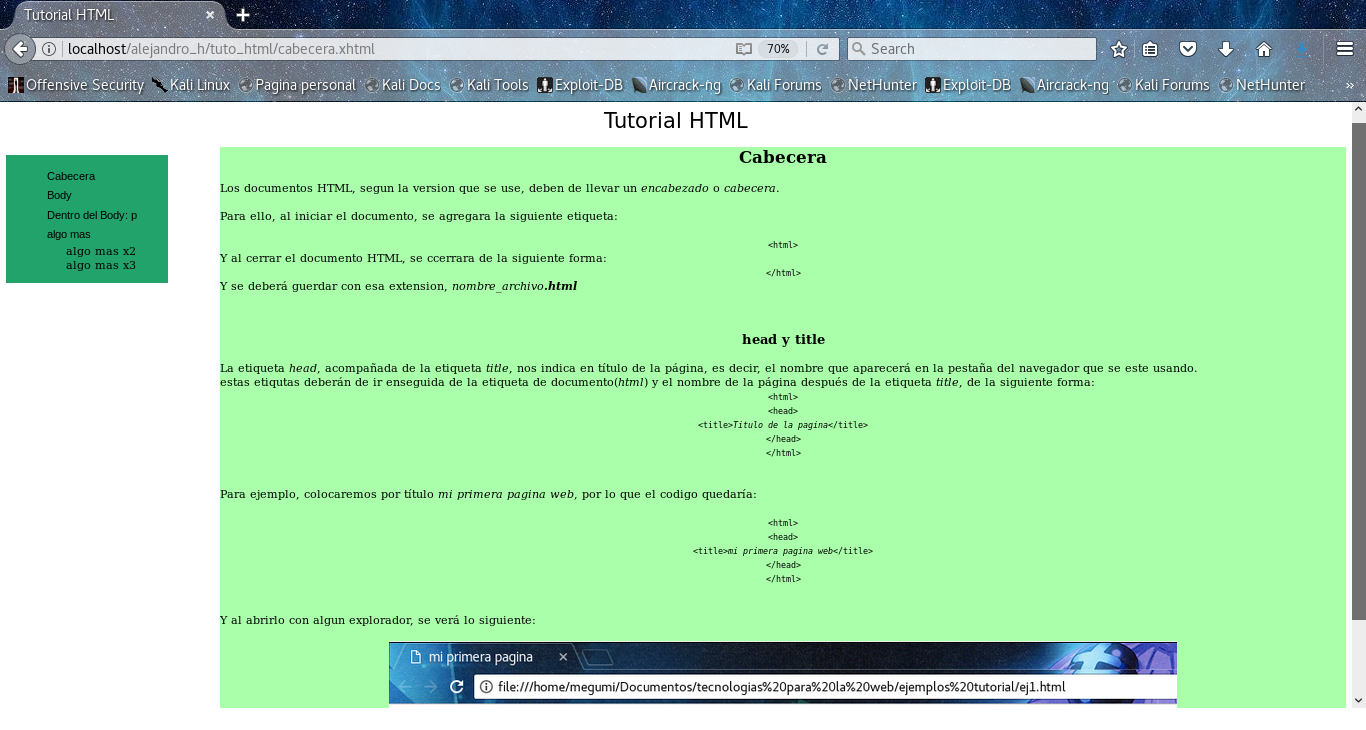
\includegraphics[scale=0.3]{./imgs/cabecera.png}
\vspace{-10mm}
{\em{\caption {cabecera}}}\label{figura 9}
\end{figure}
\end{center}
\vspace{-1cm}
Luego, vayamos al contenido de {\em body}, el cu\'al queda:
\vspace{-5mm}
\begin{center}
\begin{figure}[h!]
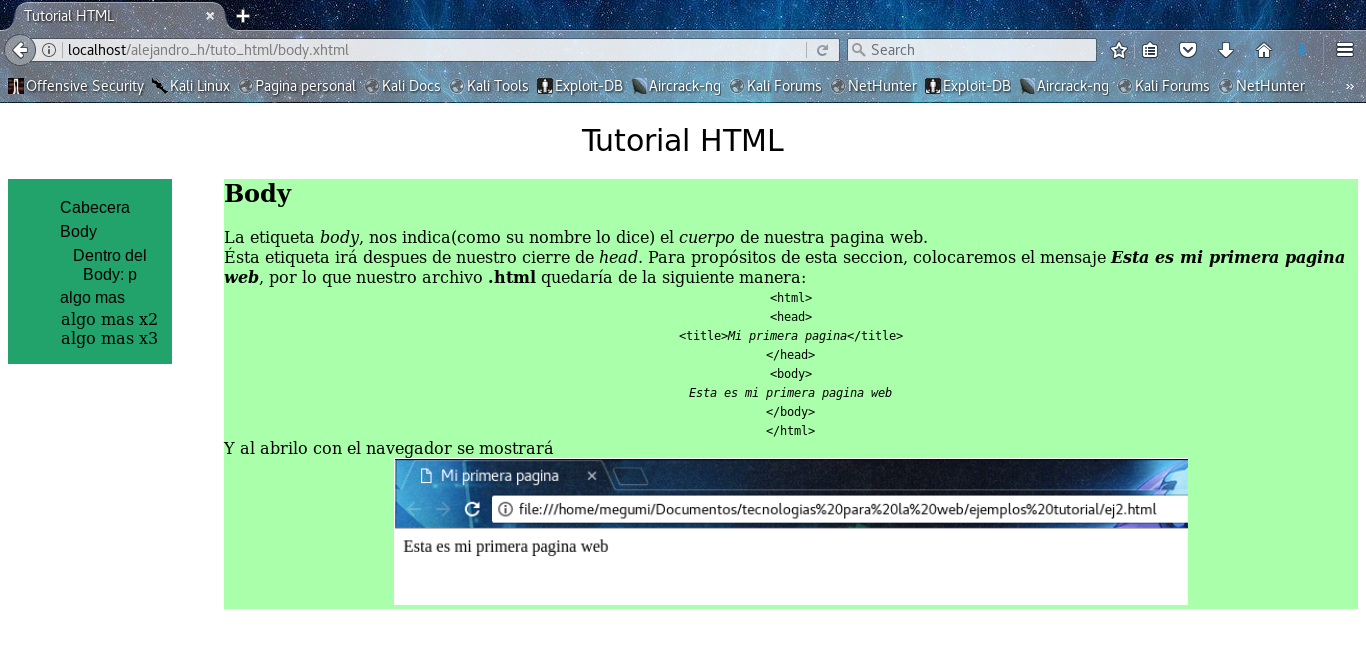
\includegraphics[scale=0.3]{./imgs/body.png}
\vspace{-10mm}
{\em{\caption {body}}}\label{figura 10}
\end{figure}
\end{center}
\vspace{-1cm}
\newpage
Ahora, vamos con la seccion {\bf {\em Dentro del body}}, el cual contiene la etiqueta \verb@<p>@
\vspace{-5mm}
\begin{center}
\begin{figure}[h!]
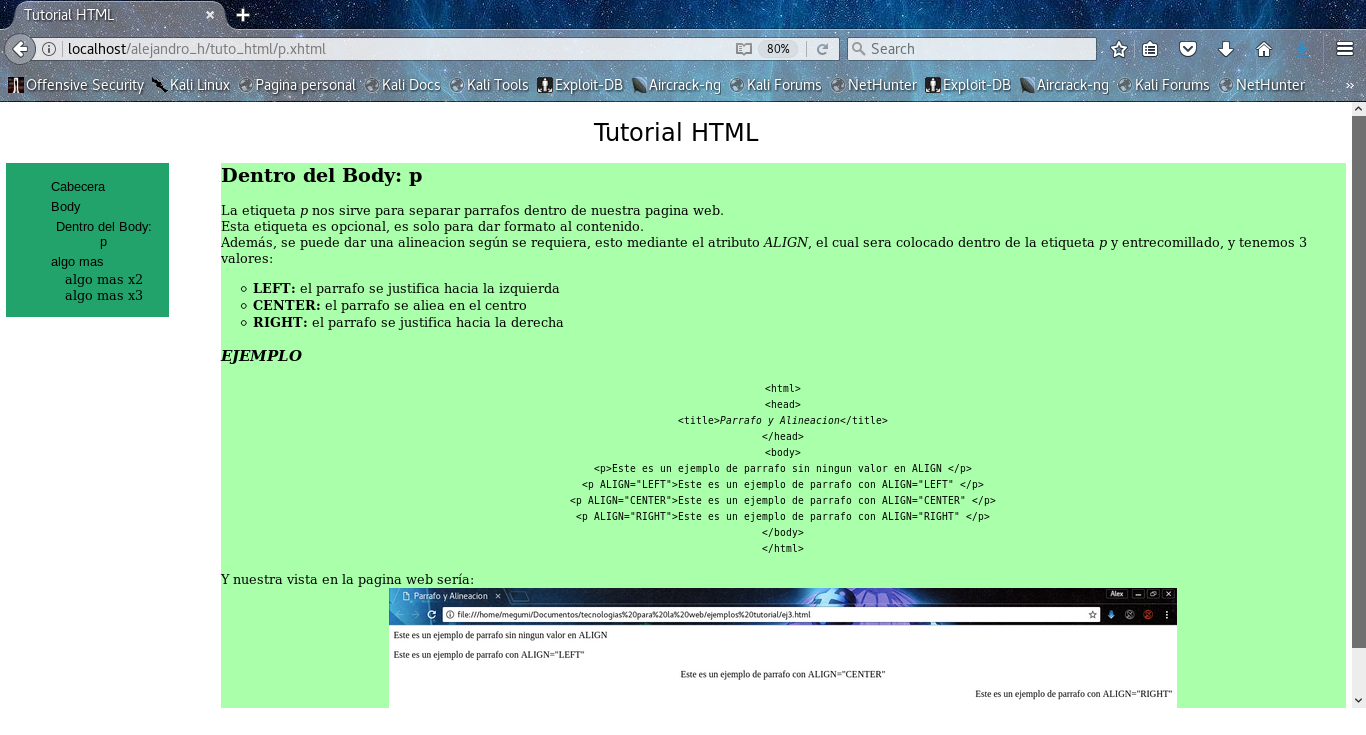
\includegraphics[scale=0.3]{./imgs/p.png}
\vspace{-10mm}
{\em{\caption {Dentro del body}}}\label{figura 11}
\end{figure}
\end{center}
\vspace{-1cm}
Entonces, nuestor directorio de archivos, desde los archivos {\bf {\em xhtml}}, los archivos {\bf {\em css}}, las imagenes, videos y demas, queda: 
\vspace{-5mm}
\begin{center}
\begin{figure}[h!]
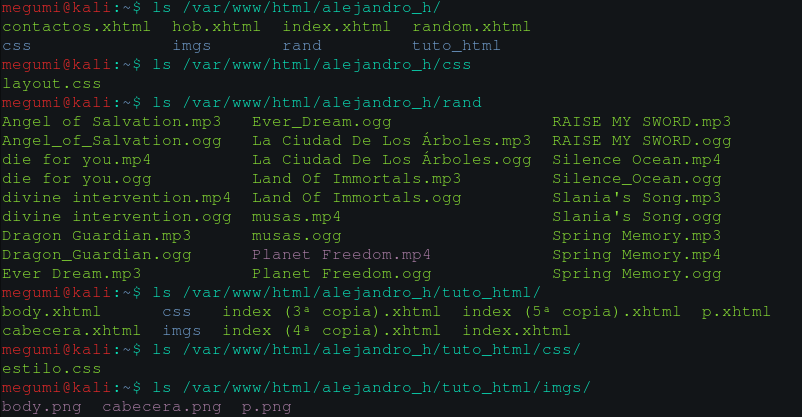
\includegraphics[scale=0.5]{./imgs/dire.png}
\vspace{-10mm}
{\em{\caption {Directorio de Archivos}}}\label{figura 12}
\end{figure}
\end{center}
\vspace{-1cm}
\newpage
{\Huge{\rm {\bf Conclusi\'on}}}
\\
\vspace{5mm}
Al principio, hacer el dise\~no en {\em html} fue bastante facil, pues podia haber etiquetas sin cerrar.\\
\vspace{5mm}
Despu\'es, al hacer la migraci\'on de {\em html} a {\em xhtml}, quiz\'as reresent\'o un peque\~no dolor de cabeza, pues las posibles etiquetas que no se cerraron, o que se cerraban "2 veces", represent\'o un problema a la hora de poder visualizar la pagina web, pues indicaba que linea estaba mal, o que posible error o errores tenia el codigo.
\\
\vspace{5mm}
Con esto queda demostrado lo estricto que es crear codigo {\em html} y guardarlo como {\em xhtml}.


\end{flushleft}

%termina documento
\end{document}